\documentclass[12pt,]{report}
\usepackage{lmodern}
\usepackage{amssymb,amsmath}
\usepackage{ifxetex,ifluatex}
\usepackage{fixltx2e} % provides \textsubscript
\ifnum 0\ifxetex 1\fi\ifluatex 1\fi=0 % if pdftex
  \usepackage[T1]{fontenc}
  \usepackage[utf8]{inputenc}
\else % if luatex or xelatex
  \ifxetex
    \usepackage{mathspec}
  \else
    \usepackage{fontspec}
  \fi
  \defaultfontfeatures{Ligatures=TeX,Scale=MatchLowercase}
\fi
% use upquote if available, for straight quotes in verbatim environments
\IfFileExists{upquote.sty}{\usepackage{upquote}}{}
% use microtype if available
\IfFileExists{microtype.sty}{%
\usepackage[]{microtype}
\UseMicrotypeSet[protrusion]{basicmath} % disable protrusion for tt fonts
}{}
\PassOptionsToPackage{hyphens}{url} % url is loaded by hyperref
\usepackage[unicode=true]{hyperref}
\PassOptionsToPackage{usenames,dvipsnames}{color} % color is loaded by hyperref
\hypersetup{
            pdftitle={Resolvendo CAPTCHAs},
            pdfauthor={Julio Trecenti},
            colorlinks=true,
            linkcolor=Maroon,
            citecolor=Blue,
            urlcolor=Blue,
            breaklinks=true}
\urlstyle{same}  % don't use monospace font for urls
\usepackage{natbib}
\bibliographystyle{apalike}
\usepackage{color}
\usepackage{fancyvrb}
\newcommand{\VerbBar}{|}
\newcommand{\VERB}{\Verb[commandchars=\\\{\}]}
\DefineVerbatimEnvironment{Highlighting}{Verbatim}{commandchars=\\\{\}}
% Add ',fontsize=\small' for more characters per line
\usepackage{framed}
\definecolor{shadecolor}{RGB}{248,248,248}
\newenvironment{Shaded}{\begin{snugshade}}{\end{snugshade}}
\newcommand{\KeywordTok}[1]{\textcolor[rgb]{0.13,0.29,0.53}{\textbf{#1}}}
\newcommand{\DataTypeTok}[1]{\textcolor[rgb]{0.13,0.29,0.53}{#1}}
\newcommand{\DecValTok}[1]{\textcolor[rgb]{0.00,0.00,0.81}{#1}}
\newcommand{\BaseNTok}[1]{\textcolor[rgb]{0.00,0.00,0.81}{#1}}
\newcommand{\FloatTok}[1]{\textcolor[rgb]{0.00,0.00,0.81}{#1}}
\newcommand{\ConstantTok}[1]{\textcolor[rgb]{0.00,0.00,0.00}{#1}}
\newcommand{\CharTok}[1]{\textcolor[rgb]{0.31,0.60,0.02}{#1}}
\newcommand{\SpecialCharTok}[1]{\textcolor[rgb]{0.00,0.00,0.00}{#1}}
\newcommand{\StringTok}[1]{\textcolor[rgb]{0.31,0.60,0.02}{#1}}
\newcommand{\VerbatimStringTok}[1]{\textcolor[rgb]{0.31,0.60,0.02}{#1}}
\newcommand{\SpecialStringTok}[1]{\textcolor[rgb]{0.31,0.60,0.02}{#1}}
\newcommand{\ImportTok}[1]{#1}
\newcommand{\CommentTok}[1]{\textcolor[rgb]{0.56,0.35,0.01}{\textit{#1}}}
\newcommand{\DocumentationTok}[1]{\textcolor[rgb]{0.56,0.35,0.01}{\textbf{\textit{#1}}}}
\newcommand{\AnnotationTok}[1]{\textcolor[rgb]{0.56,0.35,0.01}{\textbf{\textit{#1}}}}
\newcommand{\CommentVarTok}[1]{\textcolor[rgb]{0.56,0.35,0.01}{\textbf{\textit{#1}}}}
\newcommand{\OtherTok}[1]{\textcolor[rgb]{0.56,0.35,0.01}{#1}}
\newcommand{\FunctionTok}[1]{\textcolor[rgb]{0.00,0.00,0.00}{#1}}
\newcommand{\VariableTok}[1]{\textcolor[rgb]{0.00,0.00,0.00}{#1}}
\newcommand{\ControlFlowTok}[1]{\textcolor[rgb]{0.13,0.29,0.53}{\textbf{#1}}}
\newcommand{\OperatorTok}[1]{\textcolor[rgb]{0.81,0.36,0.00}{\textbf{#1}}}
\newcommand{\BuiltInTok}[1]{#1}
\newcommand{\ExtensionTok}[1]{#1}
\newcommand{\PreprocessorTok}[1]{\textcolor[rgb]{0.56,0.35,0.01}{\textit{#1}}}
\newcommand{\AttributeTok}[1]{\textcolor[rgb]{0.77,0.63,0.00}{#1}}
\newcommand{\RegionMarkerTok}[1]{#1}
\newcommand{\InformationTok}[1]{\textcolor[rgb]{0.56,0.35,0.01}{\textbf{\textit{#1}}}}
\newcommand{\WarningTok}[1]{\textcolor[rgb]{0.56,0.35,0.01}{\textbf{\textit{#1}}}}
\newcommand{\AlertTok}[1]{\textcolor[rgb]{0.94,0.16,0.16}{#1}}
\newcommand{\ErrorTok}[1]{\textcolor[rgb]{0.64,0.00,0.00}{\textbf{#1}}}
\newcommand{\NormalTok}[1]{#1}
\usepackage{longtable,booktabs}
% Fix footnotes in tables (requires footnote package)
\IfFileExists{footnote.sty}{\usepackage{footnote}\makesavenoteenv{long table}}{}
\usepackage{graphicx,grffile}
\makeatletter
\def\maxwidth{\ifdim\Gin@nat@width>\linewidth\linewidth\else\Gin@nat@width\fi}
\def\maxheight{\ifdim\Gin@nat@height>\textheight\textheight\else\Gin@nat@height\fi}
\makeatother
% Scale images if necessary, so that they will not overflow the page
% margins by default, and it is still possible to overwrite the defaults
% using explicit options in \includegraphics[width, height, ...]{}
\setkeys{Gin}{width=\maxwidth,height=\maxheight,keepaspectratio}
\IfFileExists{parskip.sty}{%
\usepackage{parskip}
}{% else
\setlength{\parindent}{0pt}
\setlength{\parskip}{6pt plus 2pt minus 1pt}
}
\setlength{\emergencystretch}{3em}  % prevent overfull lines
\providecommand{\tightlist}{%
  \setlength{\itemsep}{0pt}\setlength{\parskip}{0pt}}
\setcounter{secnumdepth}{5}
% Redefines (sub)paragraphs to behave more like sections
\ifx\paragraph\undefined\else
\let\oldparagraph\paragraph
\renewcommand{\paragraph}[1]{\oldparagraph{#1}\mbox{}}
\fi
\ifx\subparagraph\undefined\else
\let\oldsubparagraph\subparagraph
\renewcommand{\subparagraph}[1]{\oldsubparagraph{#1}\mbox{}}
\fi

% set default figure placement to htbp
\makeatletter
\def\fps@figure{htbp}
\makeatother

\usepackage[brazilian]{babel}
\usepackage[utf8]{inputenc}
\usepackage[T1]{fontenc}
\usepackage{lipsum}
\usepackage{fullwidth}
\usepackage{indentfirst}
\usepackage[left=2.5cm, right=2.5cm, top=4cm, bottom=3.8cm]{geometry}
\renewcommand{\familydefault}{\sfdefault}
\PassOptionsToPackage{dvipsnames}{xcolor}
\RequirePackage{xcolor} % [dvipsnames]
\definecolor{halfgray}{gray}{0.55} % chapter numbers will be semi transparent .5 .55 .6 .0
\definecolor{webgreen}{rgb}{0,.5,0}
\definecolor{webbrown}{rgb}{.6,0,0}
%\definecolor{Maroon}{cmyk}{0, 0.87, 0.68, 0.32}
%\definecolor{RoyalBlue}{cmyk}{1, 0.50, 0, 0}
%\definecolor{Black}{cmyk}{0, 0, 0, 0}
\usepackage{fancyhdr}
\usepackage{pdfpages}
\usepackage{amsmath}
\usepackage{graphicx}
\usepackage{listings}
\usepackage{enumitem}
\usepackage{setspace}
\usepackage{spverbatim}
\usepackage{lipsum}
\usepackage{natbib}
\usepackage{longtable}
\usepackage{booktabs}
\usepackage{background}

% \newcommand{\prestadorEmpresaFoot}{Associação Brasileira de Jurimetria}
% \newcommand{\prestadorEmpresa}{Associação Brasileira de Jurimetria}
% \newcommand{\prestadorRepr}{Marcelo Guedes Nunes}
% \newcommand{\prestadorEnderecoFoot}{Rua Gomes de Carvalho, 1356, 1º andar. CEP 04547-005 - São Paulo, SP, Brasil.}
% \newcommand{\prestadorEndereco}{Rua Gomes de Carvalho, 1356, 1º andar}
% \newcommand{\prestadorEnderecoComp}{CEP 04547-005 - São Paulo, SP, Brasil}
% \newcommand{\prestadorSite}{\url{http://abj.org.br}}
% \newcommand{\prestadorEmail}{contato@abj.org.br}
% \newcommand{\logo}{
\includegraphics[width=0.21\textwidth, trim=0cm 0cm 0cm 11.1cm, clip]{imgs/logo_abj.png}}


\setlength{\parindent}{2em}

% \backgroundsetup{
% scale=1,
% angle=0,
% opacity=1,
% color=black,
% contents={\begin{tikzpicture}[remember picture,overlay]
% \node at ([xshift=-4.35cm,yshift=-2.5cm] current page.north east) % Adjust the position of the logo.
% {\logo}; % logo goes here
% \end{tikzpicture}}
% }

\usepackage{float}
\let\origfigure\figure
\let\endorigfigure\endfigure
\renewenvironment{figure}[1][2] {
    \expandafter\origfigure\expandafter[H]
} {
    \endorigfigure
}

\title{Resolvendo CAPTCHAs}
\author{Julio Trecenti}
\date{19 de julho de 2018}

\begin{document}
\maketitle

{
\hypersetup{linkcolor=black}
\setcounter{tocdepth}{2}
\tableofcontents
}
\listoftables
\listoffigures
\chapter{Introdução}\label{introducao}

CAPTCHAs (\emph{Completely Automated Public Turing test to tell
Computers and Humans Apart}) são desafios criados com soluções fáceis de
obter por humanos, mas difíceis de obter por robôs. Os CAPTCHAs nasceram
entre 2000 e 2002 nos laboratórios da universidade de Carnegie Mellon
\citep{von2002telling}, como uma tecnologia utilizada para evitar
ataques \emph{spam}.

Ao longo dos anos, os CAPTCHAs tornaram-se comuns em diversas páginas da
internet, podendo ser encontrados a partir de desafios de visão,
audição, operações matemáticas, entre outros. Essa popularidade também
trouxe iniciativas para resolver CAPTCHAs automaticamente, a partir de
inputs humanos, heurísticas codificadas manualmente e até sistemas mais
sofisticados de inteligência artificial. A disputa entre geradores e
resolvedores gera debates profundos até os dias de hoje.

Apesar da origem na criptografia e motivação prática, pode-se argumentar
que CAPTCHAs representam um problema geral da inteligência artificial
\citep{george2017generative}.

Essencialmente, o CAPTCHA (baseado em imagens) é uma resposta natural
para pergunta de pesquisa: que aspecto da visão humana não pode ser
automatizado? Essa pergunta serve não só para criar novos CAPTCHAs mas
também para orientar a pesquisa em visão computacional.

Uma forma ad-hoc de responder à essa pergunta é criando desafios
complexos. Por exemplo, elaborando tarefas de identificar textos dentro
de imagens completamente distorcidas e cheias de ruído. No entanto, hoje
somos perfeitamente capazes de resolver esse problema com altíssima taxa
de acerto, muitas vezes mais altas que de humanos. Para isso, só
precisamos de uma base de dados de treino suficientemente grande e
modelos de aprendizado estatístico flexíveis, que chamamos de
força-bruta. Discutiremos sobre isso no Capítulo 3.

Talvez a resposta não esteja na dificuldade, mas no contexto. Ao mudar o
ambiente que circunda a tarefa, mudamos a base de dados necessária para
lidar com o problema. Como o levantamento de novas bases de dados de
treino é custosa, essa estratégia torna a resolução por métodos de
força-bruta inexequíveis. Esse racional foi a base da criação da versão
dois do \textbf{reCaptcha} da Google, amplamente utilizada nos dias de
hoje. O reCaptcha pode ser considerado o problema a ser batido nessa
área.

E de que forma podemos avançar na pesquisa? Nossa hipótese, que é o
objeto principal dessa tese, é a de que é possível desenvolver técnicas
para aumentar a eficiência e a capacidade de generalização dos modelos
para resolver CAPTCHAs baseados em textos, aproveitando ao máximo o que
existe de informação disponível no contexto de CAPTCHAs e visão
computacional. Qualquer passo positivo nesse sentido é um novo avanço na
pesquisa de resolução de CAPTCHAs e, consequentemente, em problemas mais
profundos de inteligência artificial.

A jornada a deste projeto de doutorado parte do problema geral dos
CAPTCHAs e se encerra na apresentação e avaliação de diversas abordagens
para aumentar a eficiência e a capacidade de generalização dos modelos.
No caminho, faremos uma ponte entre modelos estatísticos usuais e
modelos de redes neurais convolucionais, com o intuito de mostrar que
essencialmente estamos apenas estendendo modelos, não abandonando a
estatística clássica.

Nesse primeiro produto de qualificação, definimos o problema geral dos
CAPTCHAs e suas variantes. Em seguida, mostramos a solução clássica e a
solução força-bruta para o problema, apresentando os resultados obtidos
até o momento. Encerramos o trabalho apresentando informalmente com os
conceitos de eficiência e generalização, apontando os próximos passos
que a pesquisa deve seguir.

\section{Objetivos}\label{objetivos}

O objetivo geral dessa tese é buscar formas eficientes e gerais de
resolver CAPTCHAs de imagens baseados em textos.

Os objetivos específicos são:

\begin{itemize}
\tightlist
\item
  Definir o problema do CAPTCHA e duas variações
\item
  Mostrar uma solução força-bruta que funciona com alta taxa de acurácia
\item
  Realizar uma ponte teórica entre regressão logística e redes neurais
  convolucionais
\item
  Desenvolver uma ferramenta para resolver CAPTCHAs que seja útil e
  simples de utilizar.
\item
  Discutir e testar diversas abordagens para aumentar eficiência e
  capacidade de generalização dos modelos.
\end{itemize}

\section{Resultados esperados}\label{resultados-esperados}

O projeto de doutorado já possui novos avanços relevantes nesses pontos:

\begin{itemize}
\tightlist
\item
  Implementação colaborativa do pacote \texttt{decryptr} na linguagem R
  para resolver CAPTCHAs
\item
  Ponte teórica entre modelo de regressão logística e redes neurais
  convolucionais utilizando notação comum para estatísticos.
\item
  Levantamento de lista curada de artigos sobre o tema.
\item
  Resolução de diversos CAPTCHAs que nunca foram trabalhados no passado.
\end{itemize}

Ao final do projeto, teremos mais esses novos avanços:

\begin{itemize}
\tightlist
\item
  Implementação das metodologias mais recentes de forma reprodutível
\item
  Estudo e validação de abordagens para aumentar eficiência e
  generalização dos algoritmos
\item
  Investigação do uso de aprendizado por reforço e aproveitamento do
  oráculo
\end{itemize}

\section{Revisão bibliográfica}\label{revisao-bibliografica}

A produção acadêmica sobre CAPTCHAs se agrupa em dois tópicos: geração e
resolução. Os artigos de geração buscam as formas mais eficazes de criar
tarefas difíceis para robôs e fáceis para humanos. Já os artigos de
resolução tentam criar novos métodos para lidar com os CAPTCHAs mais
comuns da internet.

\citep{von2002telling} define captchas pela primeira vez.
\citet{von2003captcha} deduz o problema de resolver CAPTCHA a partir de
uma definição matemática genérica do problema da inteligência
artificial. \citet{mori2003recognizing} apresentam uma solução
rudimentar para o problema a partir de cortes em imagens. O modelo final
acerta somente 33\% dos casos. \citet{yan2008low} criam um modelo de
quebrar CAPTCHAs baseado em diversas heurísticas.
\citet{yan2008usability} apresentam os principais problemas de
utilização no desenvolvimento de CAPTCHAs concluindo, principalmente,
que CAPTCHAs baseados em textos podem sim ser desafios complexos.
\citet{golle2008machine} utilizam máquinas de vetor de suporte pela
primeira vez. \citet{motoyama2010re} estudam o aspecto econômico dos
reCaptchas, avaliando o impacto de sua utilização ampla em toda a
internet. \citet{bursztein2011text} testam diversos modelos em 15
captchas diferentes e concluem que a melhor forma de criar CAPTCHAs
complicados é colando as letras. \citet{bursztein2014end} mostram pela
primeira vez um modelo um modelo de aprendizado por reforço, utilizando
feedbacks humanos. \citet{george2017generative} desenvolvem um novo
modelo capaz de quebrar CAPTCHAs a partir de pouquíssimos exemplos.

\chapter{Problema}\label{problema}

A decifragem de Captchas pode ser entendida como um problema de
classificação de imagens. Especificamente, nosso interesse é criar uma
função \(g\) que recebe uma imagem
\(\mathbf X = \{x_{nmr} \in [0,1]\}_{N\times M \times R}\) e retorna um
vetor de índices \(\mathbf y\). Cada índice \(y_j\) indica a presença de
um caractere \(c_j\), \(j = 1, \dots, L\), onde \(L\) é o número de
caracteres contidos na imagem. Chamaremos \(L\) de \emph{comprimento} do
Captcha, com \(L \in \mathbb{Z}_+\).

O problema pode ser detalhado em três itens, listados abaixo:

\begin{enumerate}
\def\labelenumi{\arabic{enumi}.}
\tightlist
\item
  Nossa variável \textbf{explicativa}, a imagem, é uma matriz
  \(\mathbf X = \{x_{ijk}\}_{N\times M \times R}\), em que \(N\) é o
  número de linhas, \(M\) é o número de colunas e \(R\) é o número de
  \emph{cores}, ou \emph{canais}.
\end{enumerate}

O elemento \(x_{nm\cdot}\) é denominado \emph{pixel}. Um pixel
representa a menor unidade possível da imagem. Em uma imagem colorida,
por exemplo, temos \(R=3\). Nesse caso, um pixel é um vetor de três
dimensões com valores entre zero e um, representando a intensidade de
vermelho, verde e azul da coordenada \((n, m)\) da imagem. Numa imagem
em escala de cinza, por exemplo, temos \(R=1\) e o pixel, de uma
dimensão, representa a intensidade do cinza, sendo 1 o equivalente da
cor branca e 0 o preto.

\begin{enumerate}
\def\labelenumi{\arabic{enumi}.}
\setcounter{enumi}{1}
\item
  O objeto \(C \in \mathcal A^L\) é um vetor de itens de um alfabeto
  \(\mathcal A\), de cardinalidade \(|\mathcal A|\), finito e conhecido.
  Esse alfabeto contém todos os possíveis caracteres que podem aparecer
  na imagem.
\item
  Nossa \textbf{resposta}
  \(\mathbf y \in \mathbb \{1, \dots, |\mathcal A|\}^L\) é um vetor de
  índices de tamanho fixo. Cada elemento de \(\mathbf y\) representa um
  elemento do alfabeto \(\mathcal A\).
\end{enumerate}

A obtenção de uma função \(g\) capaz de mapear \(\mathbf y\) a partir de
uma nova imagem \(\mathbf X\) depende de uma amostra de imagens
\(\mathbf X_1, \dots, \mathbf X_S\), corretamente classificadas através
do vetor \(\mathbf y_1, \dots, \mathbf y_S\). A tarefa é, portanto,
obter uma estimativa \(\hat g\) para a função \(g\) que minimiza

\[
L(\hat g(\mathbf X), \mathbf y) = \mathbb I(g(\mathbf X) \neq \mathbf y)
\]

em que \(\mathbb I(g(\mathbf X) \neq \mathbf y)\) indica se
\(g(\mathbf X)\) difere do que é observado em \(\mathbf y\). Isto é,
pretende-se encontrar uma função que minimize a taxa de classificação
incorreta das imagens que descrevem os textos dos Captchas.

\section{Variantes}\label{variantes}

\subsection{Áudio}\label{audio}

Assim como em outros problemas, existem diversas formas de representação
de dados.\\
Para os Captchas, também é possível encontrá-los em formato de áudio.
Nestes casos, o usuário é condicionado a ouvir um áudio e transcrever o
que foi entendido de seu conteúdo em um texto.

É importante notar que este formato avalia uma competência diferente do
usuário, em comparação às imagens. Com base na avaliação de Captchas de
áudio durante o desenvolvimento do trabalho, verificou-se que estes são,
em geral, menos complexos. Por exemplo, alguns Captchas neste formato
são compostos por sons sem ruído, claramente entendíveis tanto por um
ser humano quanto por uma máquina. Ou seja, caso se queira realizar a
classificação automática destes Captchas, basta ter um conjunto de sons
com seus respectivos significados. Dessa forma, um computador pode
facilmente combinar os sons fornecidos com os correspondentes caracteres
e obter a resposta para o desafio proposto, quebrando o Captcha.

Para os casos aonde há presença de ruído no áudio, existem
fundamentalmente duas técnicas para a quebra dos Captchas. A primeira é
baseada em engenharia de características {[}ref{]}, que consiste na
extração de covariáveis referentes aos áudios, utilizadas posteriormente
em um modelo de regressão clássico para a classificação. O segundo
método trata de encontrar o espectrograma do áudio, possibilitando o
tratamento dele como uma imagem, o que nos leva a algo parecido com o
problema inicial.

\subsection{Covariáveis e número de respostas
variável}\label{covariaveis-e-numero-de-respostas-variavel}

Outra forma comum de manifestação de Captchas são imagens em que o
número de letras é variante. Esse problema é mais complexo que o
anterior, uma vez que a variável resposta não é mais um vetor de tamanho
\(L\) fixo.

Porém, é possível assumir o número de letras máximo que aparece numa
imagem como fixo. Dessa maneira, uma solução para o problema do tamanho
variável é considerar um caractere adicional \texttt{\_} no alfabeto,
chamado \emph{placeholder}, que representa a ausência do algum caractere
em determinada posição. Este caractere tem a função de substituir as
posições vazias, fazendo com que o comprimento destes Captchas seja
também uniforme. Assim, uma imagem com \(L_{\max} = 5\), por exemplo,
pode ter uma classificação \texttt{cad5\_}, que tem apenas quatro
letras, mas foi completada até o número máximo de caracteres com o
\emph{placeholder}.

Uma complicação dessa proposta é que a posição dos \emph{placeholders}
não importa na classificação do captcha. Em outras palavras, as soluções
\texttt{cad5\_}, \texttt{ca\_d5} e \texttt{\_cad5} são equivalentes.
Considerando a função de classificação a ser estimada, este obstáculo
aumenta a dificuldade na estimação dos parâmetros por gerar mais ótimos
locais, em detrimento de pontos ótimos globais.

Ainda nesta situação, outra alternativa é considerar que um dos
interesses de predição é justamente o número de letras. Assim, teríamos

\[
\tilde{\mathbf{y}} = \left[l \;\; \mathbf y^\top \right]^\top,
\]

onde \(l\) é o número de letras do Captcha específico e \(\mathbf y\)
tem comprimento \(L_{\max}\), preenchido com \emph{placeholders}, como
anteriormente. A presença do número de letras como componente da
variável resposta do problema permite trabalhar adequadamente com os
\emph{placeholders}, pois podemos descartá-los na função de perda
(verossimilhança) nas vezes em que o número de letras estimadas for
menor do que \(L_{\max}\).

Usualmente, o problema de Captchas de tamanho variável é acompanhado
pelo problema das covariáveis. Um tipo comum de Captcha com covariáveis
envolve desafios como ``digite todas as letras da cor verde''. Nesse
caso, ``verde'' é uma covariável, pois é uma das informações que deve
ser utilizada em combinação com a imagem completa para a predição
correta do texto do Captcha.

Inicialmente, pode parecer contra-intuitivo considerar uma imagem e um
texto como covariáveis para predizer o valor de \(\mathbf y\). Todavia,
isso se dá de forma natural, principalmente na solução que proposta no
Capítulo \ref{results}.

\subsection{reCaptcha 2.0}\label{recaptcha-2.0}

O reCaptcha 2.0 desenvolvido pela Google é o \emph{benchmark} no que se
refere a geração de CAPTCHAs. Nesse desafio, o usuário é colocado para
resolver diversos tipos de problemas de imagens como reconhecimento de
placas de trânsito, fachadas de prédios e carros. O reCaptcha é
utilizado não só para barrar robôs, como também para alimentar os
modelos estatísticos da própria Google para seus produtos, como, por
exemplo, o desenvolvimento de carros autônomos.

A dificuldade em resolver estes Captchas consiste na pluralidade de
contextos, não na dificuldade que eles propõem
\citep{goodfellow2013multi}. A tarefa de identificar placas de trânsito
em imagens é complicada, mas pode ser resolvida com alta taxa de
acurácia utilizando-se modelos adequados. No entanto, o reCaptcha pode
facilmente mudar a tarefa para identificação de fachadas, ou então
identificação de felinos. Do ponto de vista estatístico, cada uma dessas
tarefas exige uma base de dados de treinamento diferente, aumentando
exponecialmente a dificuldade de resolução.

Na prática, o reCaptcha cria um jogo em que o autor do CAPTCHA tem
muitas vantagens. O tempo necessário para criar uma nova tarefa é menor
que o tempo necessário para resolvê-lo. Até hoje não existe uma solução
geral para o reCaptcha 2.0 com taxas satisfatórias de acurácia. A
principal forma de contornar o reCaptcha 2.0 é através da exploração de
falhas no sistema de identificação de robôs ou a possibilidade de
receber tarefas por áudio {[}sivakorn2016m{]}. Outras abordagens
utilizam modelos robustos, como o ImageNet, para detecção genérica de
objetos nas imagens, mas sem taxas de sucesso expressivas
{[}mach2017automaticky{]}.

\chapter{Solução}\label{results}

\section{Segmentação e classificação}\label{segmentacao-e-classificacao}

Um problema de resolver o CAPTCHA diretamente é que a variável resposta
\(\mathbf y\) tem um número exponencial de combinações. Na formulação do
capítulo anterior, nossa resposta é uma palavra de \(L\) caracteres,
sendo que cada caractere \(c_j\) pode ter \(|\mathcal A|\) valores.
Nessa construção, o total de combinações é \(|\mathcal A|^L\).

Por exemplo, um CAPTCHA com \(L=6\) letras e \(|\mathcal A| = 36\)
possibilidades em cada letra (26 letras do alfabeto e 10 algarismos),
possui um total de 2.176.782.336 (\textgreater{} 2 bilhões) combinações.
Modelar essas imagens diretamente através de uma única variável resposta
categórica é inviável.

Por isso, uma forma de resolver CAPTCHAs é separando o problema em duas
tarefas: segmentar e classificar. A tarefa de segmentação consiste em
receber uma imagem com várias letras e detectar pontos de corte,
separando-a em várias imagens de uma letra. Já a classificação consiste
em receber uma imagem com uma letra e identificar o caractere
correspondente. Nesse caso, a resposta é reduzida para \(|\mathcal A|\)
categorias, que cresce linearmente e, portanto, tratável.

A literatura mostra através de estudos empíricos que a tarefa de
segmentar é mais difícil do que a tarefa de classificar
\citep{bursztein2014end}. Isso acontece porque o problema de
classificação de letras segmentadas é similar ao problema de
reconhecimento de caracteres (\emph{Optical Character Recognition},
OCR), que é amplamente estudado e pode ser considerado resolvido. A
segmentação, no entanto, é um problema em aberto e faz parte da
literatura de oclusão de objetos em visão computacional.

Por esse motivo, os desenvolvedores de CAPTCHAs de imagens baseadas em
texto têm explorado métodos de dificultar a segmentação. As principais
formas são i) colar os caracteres e ii) adicionar linhas ligando os
dígitos. Essas técnicas são combinadas com a adição de ruído e distorção
de caracteres para compor a imagem final.

Vamos usar como exemplo o CAPTCHA do Tribunal de Justiça de Minas Gerais
(TJMG). Nesse caso, temos \(L=4\) e \(|\mathcal A|=10\), apenas os dez
algarismos.

A Figura \ref{fig:tjmg1} mostra um exemplo do captcha do TJMG. Podemos
notar a utilização de distorção de catacteres e adição de linhas ligando
os dígitos como formas de evitar a resolução automática.

\begin{figure}
\centering
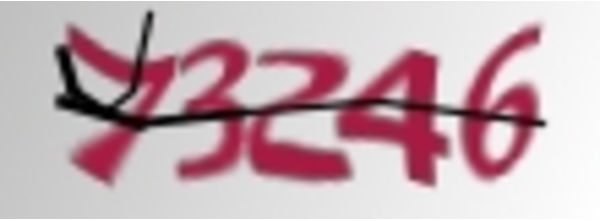
\includegraphics{jtrecenti_doctorate_captcha_files/figure-latex/tjmg1-1.pdf}
\caption{\label{fig:tjmg1}CAPTCHA do TJMG.}
\end{figure}

Nesse caso, podemos resolver o problema da segmentação realizando cortes
fixos na imagem. Podemos também limitar os eixos \texttt{x}, tirando os
espaços vazios à esquerda e à direita e \texttt{y}, removendo espaços
superiores e inferiores. Por último, transformamos a imagem em escala de
cinza. O resultado dessas operações de pré-processamento estão na Figura
\ref{fig:tjmg2}.

\begin{figure}
\centering
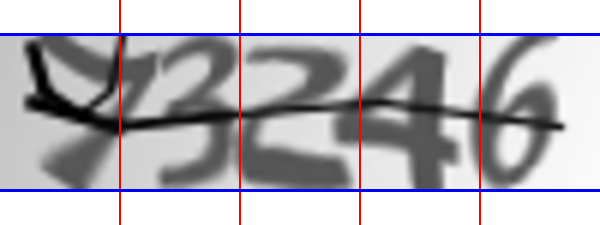
\includegraphics{jtrecenti_doctorate_captcha_files/figure-latex/tjmg2-1.pdf}
\caption{\label{fig:tjmg2}CAPTCHA do TJMG após segmentação.}
\end{figure}

O resultado são cinco imagens de dimensões \texttt{26x20}, associadas a
cada caractere. O próximo passo é transformar o banco de dados num
formato tratável por modelos tradicionais de regressão. Para isso,
colocamos cada pixel em uma coluna da nossa base de dados. No caso do
TJMG, cada CAPTCHA gera uma tabela de 5 linhas e 520
(\texttt{26\ *\ 20}) colunas. A Tabela \ref{tab:imgsep} mostra as
primeiras seis colunas dessa base.

\begin{table}

\caption{\label{tab:imgsep}Base de dados montada a partir de imagem segmentada.}
\centering
\begin{tabular}[t]{l|r|r|r|r|r|r}
\hline
y & xy01\_01 & xy01\_02 & xy01\_03 & xy01\_04 & xy01\_05 & xy01\_06\\
\hline
7 & 0.769 & 0.769 & 0.769 & 0.769 & 0.769 & 0.773\\
\hline
3 & 0.005 & 0.141 & 0.316 & 0.430 & 0.356 & 0.319\\
\hline
2 & 0.846 & 0.851 & 0.830 & 0.796 & 0.800 & 0.842\\
\hline
4 & 0.886 & 0.886 & 0.890 & 0.890 & 0.890 & 0.890\\
\hline
6 & 0.925 & 0.925 & 0.929 & 0.929 & 0.929 & 0.933\\
\hline
\end{tabular}
\end{table}

Agora basta rodar o mesmo para toda a base de treino e rodar um modelo.
Nesse exemplo, utilizamos uma base de 1500 CAPTCHAs classificados. O
resultado após o pré-processamento é uma base com 7500 linhas e 520
colunas. Escolhemos manter 6000 linhas para treino e as 1500 restantes
para teste. Utilizamos um modelo de florestas aleatórias para o exemplo
\citep{breiman2001random}.

O resultado do modelo pode ser verificado na Tabela \ref{tab:errosTJMG},
que mostra os observados \emph{versus} preditos na base de teste. O
acerto foi de 99.6\% em cada caractere. Assumindo que o erro não depende
da posição do caractere no CAPTCHA, o acerto para a imagem completa é de
aproximadamente 98\%.

\begin{table}

\caption{\label{tab:errosTJMG}Tabela de acertos e erros.}
\centering
\begin{tabular}[t]{l|l|l|l|l|l|l|l|l|l|l}
\hline
y & 0 & 1 & 2 & 3 & 4 & 5 & 6 & 7 & 8 & 9\\
\hline
0 & 156 & . & . & . & . & . & . & . & . & .\\
\hline
1 & . & 160 & . & . & . & . & . & . & . & .\\
\hline
2 & . & . & 147 & . & . & . & . & . & . & .\\
\hline
3 & . & . & 1 & 140 & . & . & . & . & . & .\\
\hline
4 & . & 2 & . & . & 150 & . & . & . & . & .\\
\hline
5 & . & . & . & . & . & 153 & . & . & . & .\\
\hline
6 & . & . & . & . & . & . & 143 & . & . & .\\
\hline
7 & . & . & . & . & . & . & . & 152 & . & .\\
\hline
8 & . & . & . & 2 & 1 & . & . & . & 139 & .\\
\hline
9 & . & . & . & . & . & . & . & . & . & 154\\
\hline
\end{tabular}
\end{table}

O resultado para o TJMG é bastante satisfatório, mas não generaliza para
outros CAPTCHAs. Tome por exemplo o CAPTCHA da Receita Federal (RFB) da
Figura \ref{fig:generalize}. Nesse caso, a posição dos caracteres muda
significativamente de imagem para imagem, e assim fica difícil cortar em
pedaços.

\begin{figure}

{\centering 
\includegraphics[width=0.32\linewidth]{jtrecenti_doctorate_captcha_files/figure-latex/generalize-1} 

}

\caption{CAPTCHA Receita Federal}\label{fig:generalize}
\end{figure}

A mesma técnica aplicada ao CAPTCHA RFB apresentou acerto de 78.8\% do
caractere, o que equivale a apenas 23.8\% de acerto para toda a imagem.
Claro que seria possível melhorar o poder preditivo com ajustes nos
hipeparâmetros do modelo, mas o problema essencial nesse caso está na
qualidade segmentação, e não na classificação dos caracteres.

Outro problema dessa técnica é que ela é incapaz de trabalhar com
CAPTCHAs de comprimento variável. Nesse caso, seria necessário construir
um modelo não supervisionado para identificar a posição das letras, o
que adiciona um grau a mais de complexidade na resolução do CAPTCHA.

Por isso, faz-se necessária uma abordagem que trabalha com problema
completo, sem passar explicitamente pela fase de segmentação. Ao invés
de cortar a imagem, vamos extrair detalhes da imagem completa
automaticamente e utilizar essas características como variáveis
preditoras num modelo de regressão. Chamaremos essa abordagem de
\emph{força bruta}.

\section{Força-bruta}\label{forca-bruta}

A abordagem de força bruta utiliza redes neurais convolucionais. Para
explicar o funcionamento dessa técnica, vamos primeiro apresentar
definições para redes neurais e para a operação de convolução. Em
seguida, vamos juntar os dois conceitos para construir o modelo
utilizado nos CAPTCHAs.

\subsection{Redes neurais}\label{redes-neurais}

Uma rede neural pode ser entendida como uma extensão de modelos lineares
generalizados com a adição de uma arquitetura aos componentes do modelo.
Para mostrar esse conceito, vamos partir da definição de um modelo
regressão logística até construir uma rede neural com camadas ocultas.

\subsubsection{Regressão logística}\label{regressao-logistica}

O modelo linear generalizado é composto por três elementos: componente
aleatório, componente sistemático e função de ligação.

O componente aleatório é uma variável aleatória com distribuição
pertencente à família exponencial, que dá origem à verossimilhança do
modelo. O componente sistemático é uma combinação linear das variáveis
preditoras com um vetor de parâmetros. A função de ligação é uma
operação que leva a componente sistemática no valor esperado da
componente aleatória. Uma forma comum de definir a ligação é propondo
uma função com domínio nos números reais e contradomínio igual ao
suporte do componente aleatório. Dessa forma, não é necessário impor
restrições aos parâmetros da componente sistemática para que os valores
ajustados variem na mesma faixa que o componente aletório.

\begin{center}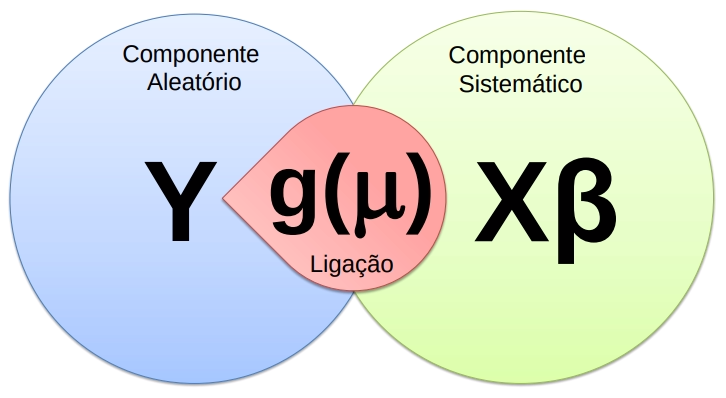
\includegraphics[width=0.4\linewidth]{imgs/glm} \end{center}

No exemplo da regressão logística, o componente aleatório tem
distribuição Bernoulli com média \(\mu\). O componente sistemático é a
combinação linear \(\mathbf X \boldsymbol \beta\) e a função de ligação
é a inversa de

\[
g(\mu) = \log\left(\frac{\mu}{1-\mu}\right)
\]

A partir de uma amostra \(y_1, \dots, y_n\) e observando que
\(\mu_i = g^{-1}(\mathbf X_i\boldsymbol\beta)\), a verossimilhança do
modelo é dada por

\[
\mathcal L(\boldsymbol \beta|\mathbf y) = \prod_{i=1}^n f(y_i|\boldsymbol\beta) = \prod_{i=1}^n\mu_i^{y_i}(1-\mu_i)^{1-y_i}
\]

A log-verossimilhança é dada por

\[
l(\boldsymbol \beta|\mathbf y) = \sum_{i=1}^n y_i\log(\mu_i) + (1-y_i)\log(1-\mu_i)
\]

Uma forma útil de olhar para a verossimilhança é a partir da
\emph{função desvio}, dada por

\[
D(\mathbf y|\boldsymbol \beta) = l(\mathbf y|\mathbf y) - l(\boldsymbol \beta|\mathbf y),
\]

onde \(l(\mathbf y|\mathbf y)\) é a verossimilhança do modelo saturado,
ou seja, calculada com \(\mathbf y\) no lugar de \(\boldsymbol \mu\). A
partir de um modelo ajustado, a função desvio pode ser interpretada como
a distância entre a verossimilhança do modelo ajustado e a
verossimilhança do modelo com um parâmetro para cada observação.

Uma propriedade interessante da função desvio é que ela equivale à
divergência de Kullback-Leibler. Por exemplo, para duas variáveis
aleatórias com distribuição Bernoulli de parâmetros \(p\) e \(q\),
respectivamente, a divergência de Kullback-Leibler é dada por

\[
D_{KL}(p||q) = p\log\left(\frac p q\right) + (1-p)\log\left(\frac{1-p}{1-q}\right)
\]

É fácil ver que

\[
\begin{aligned}
D(\mathbf y|{ \boldsymbol \beta}) &= \sum_{i=1}^n y_i\log(y_i) + (1-y_i)\log(1-y_i) - \sum_{i=1}^n y_i\log(\mu_i) + (1-y_i)\log(1-\mu_i) \\
&=\sum_{i=1}^ny_i\log\left(\frac{y_i}{\mu_i}\right) + (1-y_i)\log\left(\frac{1-y_i}{1-\mu_i}\right) \\
&= \sum_{i=1}^n D_{KL}(y_i||\mu_i) \\
&= D_{KL}(\mathbf y||{\boldsymbol\mu}).
\end{aligned}
\]

Outra propriedade interessante é que o desvio identifica unicamente a
verossimilhança do modelo. De fato, podemos reformular a definição do
modelo linear generalizado a partir da especificação do desvio ou da
divergência de Kullback-Leibler no lugar do componente aleatório. Essa
propriedade será útil na comparação com redes neurais.

Os estimadores de máxima verossimilhança de \(\boldsymbol \beta\) são os
mesmos que minimizam a função desvio. Graças à concavidade da
divergência de Kullback-Leibler, Isso pode ser feito igualando os
componentes do gradiente do desvio a zero e isolando os valores de
\(\boldsymbol \beta\):

\[
\nabla_{\boldsymbol \beta} D(\mathbf y|{ \boldsymbol \beta}) = \mathbf 0
\]

Como não é possível realizar essa operação analiticamente, utilizamos
métodos iterativos. Existem dois principais métodos iterativos
concorrentes: a descida de gradiente e o método de Newton-Raphson. No
paradigma de modelos lineares generalizados, o método de Newton-Raphson
é mais comum pois i) ele utiliza a segunda derivada e converge mais
rápido que o método da descida de gradiente, que utiliza somente a
primeira e ii) é possível demonstrar que ele equivale à aplicação
iterada de \emph{mínimos quadrados ponderados}, o que facilita
significativamente a implementação da solução. No paradigma de redes
neurais, a descida de gradiente é mais comum por conta das vantagens
\emph{backpropagation}, que veremos na próxima subseção.

Em resumo, podemos concluir que

\begin{enumerate}
\def\labelenumi{\arabic{enumi}.}
\tightlist
\item
  Um modelo linear generalizado pode ser definido por três componentes:
  a divergência de Kullback-Leibler, o preditor linear e a função de
  ligação.
\item
  A estimação dos parâmetros do modelo é realizada via descida de
  gradiente ou Newton-Raphson.
\end{enumerate}

Em seguida, veremos que a rede neural aparece quando utilizamos o
componente sistemático e a função de ligação várias vezes.

\subsubsection{Extensão para redes
neurais}\label{extensao-para-redes-neurais}

Uma forma de estender o modelo linear generalizado é considerando que o
resultado da função de ligação aplicada ao componente sistemático é uma
nova covariável \(z\). Assim, temos

\[
\begin{aligned}
\mathbf z &= g^{-1}(\mathbf X \boldsymbol \beta)\\
\boldsymbol\mu &= g^{-1}(\alpha_2\mathbf 1 + \beta_2 \mathbf z) = g^{-1}([\mathbf 1\;\mathbf z]\boldsymbol\beta_2),
\end{aligned}
\]

em que \(\boldsymbol\beta_2 = [\alpha_2\;\beta_2]^{\top}\). Agora,
podemos aumentar o número de covariáveis \(\mathbf z\) para \(k\)
covariáveis, de modo que

\[
\begin{aligned}
\mathbf z_j &= g^{-1}(\mathbf X \boldsymbol \beta_1^j)\\
\boldsymbol\mu &= g^{-1}(\mathbf Z\boldsymbol\beta_2),
\end{aligned}
\]

onde \(\mathbf Z = [\mathbf 1\;\mathbf z_1\;\dots\;\mathbf z_k]\). O
modelo espeficiado dessa forma também é chamado de \emph{multilayer
perceptron}, ou MLP.

Mesmo com essa mudança, função desvio permanece a mesma, já que
construída a partir de \(\boldsymbol \mu\). A única diferença é que
agora ela é uma função de \(\boldsymbol \beta_1^j\), \(j=1,\dots,k\) e
\(\beta_2\). O ajuste do modelo é realizado da mesma forma:

\[
\nabla_{\{\boldsymbol \beta_1^1, \dots,\boldsymbol \beta_1^k,\boldsymbol \beta_2\}} D(\mathbf y|{ \boldsymbol \beta_1^1, \dots,\boldsymbol \beta_1^k,\boldsymbol \beta_2}) = \mathbf 0
\]

A vantagem dessa extensão é que adicionamos não linearidade ao modelo.
Isso nos permite modelar relações mais complexas entre as preditoras e a
resposta, o que pode resultar em melhores predições. De fato, é possível
demonstrar que uma rede neural com uma camada oculta pode estima
qualquer função contínua entre \(\mathbf X\) e \(\mathbf y\). A
desvantagem é que a estimação via Newton-Raphson é complicada de
calcular.

É nesse momento que aparecem as vantagens da descida de gradiente.
Primeiro, defina
\(\boldsymbol \beta = \{\boldsymbol \beta_1^1, \dots,\boldsymbol \beta_1^k,\boldsymbol \beta_2\}\).
Utilizando a regra da cadeia, a derivada parcial da função desvio em
relação a \(\beta_{1,l}^{j}\) é dado por

\[
\frac{\partial D(\mathbf y|\boldsymbol\beta)}{\partial \beta_{1,l}^{j}} = \sum_{i=1}^n\frac{\partial D(\mathbf y|\boldsymbol\beta)}{\partial z_{j,i}} \frac{\partial z_{j,i}}{\partial \beta_{1,l}^{j}} .
\]

As derivadas em relação aos elementos de \(\boldsymbol \beta_2\) ocorrem
diretamente, como na especificação em apenas um nível. Todas essas
derivadas são fáceis de calcular e têm forma analítica definida. A
aplicação da regra da cadeia de forma iterada nesse contexto é chamada
de \emph{backpropagation}.

\subsubsection{Sinônimos e
generalizações}\label{sinonimos-e-generalizacoes}

A literatura de redes neurais costuma trocar o nome função de ligação
por \emph{ativação}. Isso ocorre por motivos históricos, já que as redes
neurais foram inicialmente inspiradas na ativação de sinapses de
neurônios. No contexto de redes neurais, o objetivo da função de
ativação não é, necessariamente, modificar a faixa de variação do
contradomínio, pois o resultado após a função pode ser uma nova
covariável. Isso sugere a existência de certa liberdade na escolha de
ativações. A única restrição é que a função de ativação deve ser não
linear, pois, se fosse linear, a aplicação de várias camadas de funções
resultaria numa única combinação linear. As ativações mais populares são
aquelas que têm derivadas simples.

Já a verossimilhança ou o desvio são substituídos por uma \emph{função
de perda}. A natureza probabilística do modelo é considerada
indiretamente através da função desvio, como vimos anteriormente. No
entanto, ao invés de trabalhar com o desvio, os pesquisadores de redes
neurais definem genericamente uma função de perda que mensura uma
discrepância entre os valores observados e estimados. Uma escolha
razoável de função de perda é a própria divergência de Kullback-Leibler,
calculada com base no suporte da variável resposta, gerando a função
desvio. No entanto, dependendo da aplicação, podemos escolher outras
perdas, que podem gerar distribuições de probabilidades sem formato
analítico específico.

Por último, a aplicação de camadas de não-linearidades podem ser
representadas através de um grafo direcionado acíclico. Essa
representação é vantajosa por dois motivos. O primeiro é que a aplicação
facilita a especificação e entendimento do modelo e seus parâmetros, que
podem ficar com notação carregada na especificação por fórmulas
matemáticas. A segunda é que é possível utilizar conhecimentos de teoria
dos grafos para aumentar a eficiência dos algoritmos. Por exemplo, é
possível aproveitar parte dos cálculos do \emph{backpropagation} na
obtenção das derivadas parciais da função de perda
\citep{abadi2016tensorflow}.

Em resumo, podemos concluir que

\begin{enumerate}
\def\labelenumi{\arabic{enumi}.}
\tightlist
\item
  Uma rede neural é uma extensão de modelos lineares generalizados que
  aplica combinações lineares e funções de ligação de forma iterada.
\item
  A estimação dos parâmetros é realizada por descida de gradiente,
  explorando as vantagens do backpropagation.
\item
  Funções de ligação são chamadas de funções de ativação.
\item
  A função desvio é substituída por funções de perda mais gerais.
\item
  A aplicação iterada de operações pode ser representada por um grafo
  direcionado acíclico.
\end{enumerate}

Existem diversas formas de definir, desenhar e apresentar os conceitos
básicos de redes neurais e a descida de gradiente. As melhores são
apresentadas em blogs, vídeos e aplicativos, onde as operações são
apresentadas de forma interativa. O racional apresentado nesse texto
buscou mostrar a relação intrínseca entre a regressão logística e as
redes neurais.

\subsection{A operação de convolução}\label{a-operacao-de-convolucao}

Convolução em imagens é uma operação usada nas áreas de \emph{visão
computacional} e \emph{processamento de sinais}. Ela é utilizada para
detectar padrões e aplicar filtros em imagens. Na prática, o que ela faz
é calcular um novo valor para um pixel na posição \((i,j)\) de uma
imagem com base nos valores dos pixels da vizinhança.

Uma forma organizada de fazer essa soma ponderada é criando uma matriz
de pesos. Com ela, não é necessário procurar os pontos da vizinhança.
Para cada ponto \((i,j)\), obtemos a matriz de vizinhança, multiplicamos
pontualmente pela matriz de pesos e somamos os valores resultantes.
Chamaremos essa matriz de pesos de \textbf{kernel}.

Considere

\[
K = \left[\begin{array}{rrr}-1&-1&-1\\0&0&0\\1&1&1\end{array}\right]
\]

e a seguinte imagem:

\begin{center}
\includegraphics[width=0.3\linewidth]{jtrecenti_doctorate_captcha_files/figure-latex/unnamed-chunk-3-1} \end{center}

Tome por exemplo o ponto \((i,j) = (12,16)\). A vizinhança 3x3 em torno
desse ponto é dada por

\[
P_{i,j} = \left[\begin{array}{rrr}
0.98 & 0.53 & 0.79 \\ 
0.97 & 0.99 & 1.00 \\ 
0.98 & 1.00 & 1.00 
\end{array}\right]
\]

A operação de convolução é feita da seguinte forma:

\[
\begin{aligned}
(P_{12,16} *K )_{12,16}
&= k_{1,1}p_{11,15} + k_{1,2}p_{11,16} + k_{1,3}p_{11,17} + \\
&+ k_{2,1}p_{12,15} + k_{2,2}p_{12,16} + k_{2,3}p_{12,17} + \\
&+ k_{3,1}p_{13,15} + k_{3,2}p_{13,16} + k_{3,3}p_{13,17}
\end{aligned}
\]

Esse é o valor a ser colocado no ponto \((i,j)\). Isso funciona em todos
os pontos que não estão na borda da imagem.

Existem duas formas de trabalhar com as bordas da imagem. A primeira é
preenchendo as bordas com zeros, de forma a considerar apenas os pontos
da imagem. A segunda é descartar os pontos da borda e retornar uma
imagem menor, contendo somente os pixels em que foi possível aplicar
todo o kernel.

No nosso caso, o resultado da convolução fica como na Figura
\ref{fig:emoji-horiz}. Essa matriz não foi escolhida por acaso. Ela
serve para destacar padrões horizontais da imagem. Como a primeira linha
é formada \texttt{-1}s e a última é formada por \texttt{1}s, a matriz
fica com valor alto se a parte de cima do pixel for preta e a parte de
baixo for branca (\texttt{grande\ *\ 1\ +\ pequeno\ *\ (-1)}). A parte
destacada da imagem acabou sendo os olhos (pois temos maior concentração
de pixels pretos ali), além das extremidades superior e inferior do
rosto.

\begin{figure}

{\centering 
\includegraphics[width=0.3\linewidth]{jtrecenti_doctorate_captcha_files/figure-latex/emoji-horiz-1} 

}

\caption{Figura após aplicação de convolução.}\label{fig:emoji-horiz}
\end{figure}

Aplicando o kernel vertical

\[
K = \left[\begin{array}{rrr}-1&0&1\\-1&0&1\\-1&0&1\end{array}\right],
\]

a parte destacada do rosto são as extremidades dos lados:

\begin{center}
\includegraphics[width=0.3\linewidth]{jtrecenti_doctorate_captcha_files/figure-latex/unnamed-chunk-4-1} \end{center}

A aplicação de convoluções em CAPTCHAs é direta. Nesse caso, vamos
adicionar uma constante numérica ao resuldado da convolução. Isso pode
auxiliar na visualização, pois controlamos os valores que ficam dentro
do intervalo \([0,1]\). Mais adiante veremos que esse será o intercepto
da regressão.

Vamos partir do CAPTCHA da RFB abaixo

\begin{center}
\includegraphics{jtrecenti_doctorate_captcha_files/figure-latex/unnamed-chunk-5-1} \end{center}

Esse é o resultado de adicionar o kernel vertical e bias de
\texttt{0.6}.

\begin{center}
\includegraphics{jtrecenti_doctorate_captcha_files/figure-latex/unnamed-chunk-7-1} \end{center}

Em seguida observamos o kernel horizontal. Note que identificamos
padrões das linhas horizontais que tentam atrapalhar a visão das letras.

Também vamos introduzir uma função chamada \textbf{ReLu}. ReLu significa
\emph{Restricted Linear Unit} e é uma função que zera tudo o que é
negativo e mantém tudo aquilo que é positivo inalterado. Ou seja,

\[
ReLu(x) = \frac{x + |x|}{2}
\]

ReLu não é útil para visualização da imagem, pois a substituição de
valores negativos por zero já é feita automaticamente. No entanto,
podemos aplicar várias convoluções iteradamente e separá-las por
aplicações da função ReLu. Como a função ReLu é não linear, essa
iteração gera resultados que não seriam possíveis de obter somente com
aplicações da operação convolução.

Na prática, o que queremos é treinar os valores do kernel aplicado,
buscando obter imagens transformadas que aumentem o poder preditivo.
Nesse sentido, a aplicação de convoluções, soma de constantes e ReLu são
as operações que substituem a multiplicação de matrizes, adição de
intercepto e aplicação da função de ligação na regressão logística,
respectivamente. Ou seja, uma rede neural convolucional é apenas uma
forma diferente de implementar os conceitos.

\subsection{Redes neurais
convolucionais}\label{redes-neurais-convolucionais}

Considere uma observação de uma imagem com 2x2 pixels abaixo. Note que
se o interesse for utilizar essa matriz numa regressão logística,
teríamos uma linha de nossa base de dados, com nove colunas. Ou seja, a
regressão teria nove parâmetros associados.

\[
P = \left[\begin{array}{rrr}
p_{11} & p_{12} & p_{13} \\ 
p_{21} & p_{22} & p_{23} \\
p_{31} & p_{32} & p_{33}
\end{array}\right]
\]

Considere agora o kernel \(W\), também 3x3:

\[
K = \left[\begin{array}{rrr}
k_{11} & k_{12} & k_{13} \\ 
k_{21} & k_{22} & k_{23} \\
k_{31} & k_{32} & k_{33}
\end{array}\right]
\]

A operação convolução resulta numa nova matriz 3x3, em que cada elemento
é uma combinação linear de elementos de \(P\) e \(K\). De fato, é
possível mostrar que o resultado da convolução é o resultado de uma
multiplicação de matrizes obtida através da \emph{matriz circulante} de
\(K\) \citep{gray2006toeplitz}. Ou seja, nesse caso, estamos fazendo uma
nova regressão logística, mas com os valores dos dados modificados.

Se, ao invés disso, considerarmos a matriz 2x2,

\[
K = \left[\begin{array}{rr}
k_{11} & k_{12}\\ 
k_{21} & k_{22}
\end{array}\right]
\]

estamos na prática reduzindo o problema de regressão logística para
apenas quatro parâmetros.

O modelo força-bruta é uma adaptação do clássico modelo LeNet-5
\citep{lecun2015lenet}. Esse modelo aplica convolução 3 vezes
consecutivas, adicionando o viés e a função ReLu em cada nível. Após
cada convolução, também aplicamos uma operação chamada \emph{max
pooling}, que reduz a resolução da imagem, tomando o valor máximo da
vizinhança de cada ponto. Após a aplicação das convoluções, as imagens
são remodeladas no formato retangular padrão (uma linha por imagem) e
aplicamos duas camadas de redes neurais comuns, como vimos
anteriormente.

Após a realização de todas as operações, os números resultantes não
estão entre zero e um. Por isso, aplicamos a ativação \emph{softmax},
que é a generalização da ativação logística, mas para uma resposta com
vários resultados possíveis

\[
softmax(x_i) = \frac{e^{x_i}}{\sum_ie^{x_i}}
\]

Em resumo, as operações que realizamos na rede neural convolucional são

\begin{enumerate}
\def\labelenumi{\arabic{enumi}.}
\tightlist
\item
  Tomar o input inicial (imagem).
\item
  Multiplicar (convoluir) por matrizes de pesos \(W\).
\item
  Adicionar um viés (ou intercepto) \(b\).
\item
  Aplicar uma função de ligação (ou ativação), por exemplo ReLu.
\item
  Reduzir a resolução do resultado.
\item
  Voltar para 2 várias vezes.
\item
  Tomar os pesos finais e normalizar (usando a operação \emph{softmax})
  para obter probabilidades dos resultados.
\end{enumerate}

\subsection{Resultados}\label{resultados}

Até o momento, aplicamos os modelos de redes neurais convolucionais para
cinco CAPTCHAs distintos. Os modelos foram treinados a partir de bases
de treino com aproximadamente dez mil exemplos para cada CAPTCHA. Os
resultados da aplicação dos modelos estão na Tabela
\ref{tab:resultados}. Essas taxas foram calculadas com base em 100 novos
CAPTCHAs baixados da internet após o ajuste do modelo. Podemos observar
que as taxas de acerto são todas muito próximas de 100\%. No mínimo
essas taxas estão muito próximas do que seres humanos conseguiriam
acertar.

\begin{table}

\caption{\label{tab:resultados}Resultados da aplicação dos modelos.}
\centering
\begin{tabular}[t]{l|l|l}
\hline
Imagem & Nome & Taxa de acerto\\
\hline
imgs/rfb.png & RFB & 98\%\\
\hline
![](imgs/trt.png) & TRT & 98\%\\
\hline
![](imgs/tjmg.jpeg) & TJMG & 100\%\\
\hline
![](imgs/rsc.png) & RSC & 99\%\\
\hline
![](imgs/cadesp.png) & CADESP & 98\%\\
\hline
\end{tabular}
\end{table}

Os resultados positivos da aplicação dos modelos força-bruta pode
motivar a pergunta: o problema está completamente resolvido? De fato,
podemos dizer que CAPTCHAs de imagem baseados em textos são problemas
resolvidos, desde que exista uma base de dados classificada. No entanto,
esses modelos não funcionam para novos CAPTCHAs e também erram se
fizermos pequenas alterações nas imagens. Veremos mais detalhes desse
problema no próximo capítulo.

\chapter{Eficiência e generalização}\label{eficiencia-e-generalizacao}

A modelagem via redes neurais convolucionais apresenta resultados
satisfatórios, mas tem dois problemas: eficiência e generalização.

O problema de eficiência está relacionado com o fato de que a quantidade
de imagens classificadas necessária para obter bom poder preditivo é
alta. A partir de nossos testes, identificamos que são necessários em
torno de dez mil imagens classificadas para obter um modelo com taxa de
acerto maior que 90\%.

Já o problema de generalização implica que um modelo ajustado para um
tipo CAPTCHA não funciona para outro, ainda que esses tipos sejam muito
similares. Na verdade, esses modelos sofrem do problema de
\emph{aprender} versus \emph{decorar} \citep{zhang2016understanding}.
Isso significa que pequenas modificações na imagem original,
e.g.~inclusão de ruído gaussiano na imagem, podem resultar em predições
completamente diferentes.

Os dois problemas não são independentes. Se criarmos um modelo que
generaliza, é razoável afirmar que a quantidade de dados necessária para
se obter bom poder preditivo numa nova imagem se reduz.

A Tabela \ref{tab:solucoes} mostra algumas possíveis abordagens para
resolver esses problemas.

\begin{table}

\caption{\label{tab:solucoes}Possíveis soluções para problemas de eficiência e generalização.}
\centering
\begin{tabular}[t]{l|l}
\hline
Eficiência & Generalização\\
\hline
Feedback & Ensemble\\
\hline
Reciclagem & Ruído\\
\hline
Enriquecimento & \\
\hline
\end{tabular}
\end{table}

A \textbf{reciclagem} consiste na aplicação de métodos de \emph{data
augmentation} usuais em processamento de imagens. Esses métodos
consistem em gerar novas imagens a partir das imagens originais, mas
adicionando rotações, reflexões e diferentes níveis de zoom. A vantagem
da reciclagem é a possibilidade de aumentar a base de treino sem
aumentar a quantidade de classificações manuais, o que em tese aumenta a
eficiência do aprendizado do modelo.

A aplicação de \textbf{ruídos} na imagem segue o mesmo princípio da
reciclagem, mas tem foco na generalização. Ruídos podem ser adicionados
através de distorções da imagem, ruídos aleatórios e oclusões. O ruído
adiciona robustez nas predições, o que em tese possibilitaria que um
modelo implementado para um CAPTCHA específico possa ser utilizado para
um caso similar.

A utilização de técnicas de \textbf{ensemble} visa compartilhar os
parâmetros de um modelo de CAPTCHA em outro modelo. A arquitetura
moderna de redes neurais possibilita o encaixe de modelos pré-treinados
em novas bases de treino. Por exemplo, é possível aproveitar as camadas
de redes convolucionais do captcha RFB como inputs adicionais para
modelo do TRT. Esses parâmetros podem ser considerados fixos ou podem
entrar na verossimilhança do modelo e ser atualizado. Em tese, isso
permitiria a criação de apenas um grande modelo para resolver todos os
CAPTCHAs.

O \textbf{enriquecimento} surge do fato de que origem de novos
parâmetros a serem adicionados a um modelo não precisam ser de CAPTCHAs
ajustados anteriormente. Esses parâmetros podem vir de ferramentas
genéricas de reconhecimento de caracteres (OCR) ou mesmo de bases de
dados de caracteres. \citet{george2017generative} realizaram essa
investigação com resultados satisfatórios e conseguiram reduzir o
tramanho da base de treino significativamente.

Um mecanismo de \textbf{feedback} é uma técnica usada de aumentar a
eficiência do modelo ao adicionar informações ao modelo quando a
predição falha. As informações são incluídas no modelo através de
técnicas de aprendizado por reforço \citep{sutton1998introduction}.

Existem duas formas de implementar mecanismos de feedback: automática e
manual.

A forma automática aproveita as vantagens da existência de um
\emph{oráculo} de baixo custo para aumentar o tamanho da base de dados
automaticamente. O oráculo é uma função que recebe uma imagem e uma
predição e informa se a predição está correta ou incorreta. O oráculo
tem custo baixo de utilização pois existe em praticamente todos os sites
da internet, pois geralmente o CAPTCHA está associado a um formulário de
consulta (e.g.~uma consulta processual), que verifica se o CAPTCHA foi
corretamente resolvido. O problema do oráculo é que, quando algoritmo
erra, não sabemos quais são as letras que foram preditas incorretamente.
Por exemplo, num caso com \(L=6\) letras e \(|\mathcal A|=35\), a
informação que o oráculo passa quando o algoritmo erra é que o valor
correto do CAPTCHA não é uma das \(36^6\) possibilidades. Além disso, em
muitos sites só é possível testar a predição do CAPTCHA uma vez. Isso
sugere que a informação do oráculo deve ser aliada a heurísticas para
que seja útil.

A forma manual utiliza a análise de humanos para inclusão de informações
sobre cortes da imagem e erro das letras \citep{bursztein2014end}. Uma
pergunta de pesquisa interessante nesse sentido seria: qual é a mínima
intervenção suficiente para fazer o modelo aprender? Isso pode ser
resolvido testando diversos inputs manuais e comparar o tempo de
realização do feedback com o ganho em poder preditivo.

\section{Próximos passos}\label{proximos-passos}

Na tese de doutorado, vamos utilizar reciclagem, adição de ruídos,
ensemble e enriquecimento para construir modelos mais eficientes e
robustos. Pretendemos testar os impactos dessas técnicas na relação
entre tamanho da base de treino e poder preditivo do modelo.

O grande desafio da pesquisa será a investigar a forma automatizada de
feedback. Caso seja possível evitar completamente o input humano para
resolver os CAPTCHAs, o problema de aprendizado de CAPTCHAs baseados em
texto estará completamente resolvido. Se não, vamos estudar quais são os
limites da aplicação automatizada e buscar métodos que misturem
eficientemente as duas formas de feedback.

\clearpage

\appendix \addcontentsline{toc}{chapter}{\appendixname}


\chapter{Pacote decryptr}\label{pacote-decryptr}

Uma da nossas iniciativas principais nesta tese é a criação do
\href{https://github.com/decryptr/decryptr}{pacote decryptr}. Abaixo
mostramos como usar algumas das funções principais desse pacote.

Até o momento o \texttt{decryptr} possui as seguintes restrições:

\begin{enumerate}
\def\labelenumi{\arabic{enumi}.}
\tightlist
\item
  Apenas imagens \texttt{jpg} ou \texttt{png}.
\item
  Uma imagem possui apenas números e letras.
\item
  A quantidade de caracteres de um CAPTCHA é fixa.
\item
  Dois CAPTCHAs de mesma origem têm sempre as mesmas dimensões.
\end{enumerate}

O \texttt{decryptr} ainda não está no CRAN. Isso significa que para
instalá-lo é necessário utilizar o \texttt{devtools}:

\begin{Shaded}
\begin{Highlighting}[]
\NormalTok{devtools}\OperatorTok{::}\KeywordTok{install_github}\NormalTok{(}\StringTok{'decryptr/decryptr'}\NormalTok{)}
\end{Highlighting}
\end{Shaded}

\section{\texorpdfstring{Funções do
\texttt{decryptr}}{Funções do decryptr}}\label{funcoes-do-decryptr}

As funções principais do \texttt{decryptr} são

\begin{itemize}
\tightlist
\item
  \texttt{download\_captcha()}: baixar imagens da web.
\item
  \texttt{read\_captcha()}: adicionar metadados úteis a uma string com o
  caminho do CAPTCHA.
\item
  \texttt{load\_captcha()}: carregar a imagem na memória.
\item
  \texttt{plot.captcha()}: método \texttt{S3} para desenhar o CAPTCHA na
  tela.
\item
  \texttt{classify()}: método \texttt{S3} para classificar CAPTCHAs
  manualmente.
\item
  \texttt{load\_model()}: carregar um modelo já ajustado e armazenado no
  pacote \texttt{decryptrModels}
\item
  \texttt{train\_model()}: método \texttt{S3} para ajustar um modelo
  baseado em LeNet-5 para os CAPTCHAs.
\item
  \texttt{decrypt()}: método \texttt{S3} para classificar um CAPTCHA a
  partir de um modelo ajustado e um caminho de imagem.
\end{itemize}

\subsection{Fluxo de utilização}\label{fluxo-de-utilizacao}

O modo de uso planejado do \texttt{decryptr} está descrito na Figura
\ref{fig:fluxo}.

\begin{figure}

{\centering 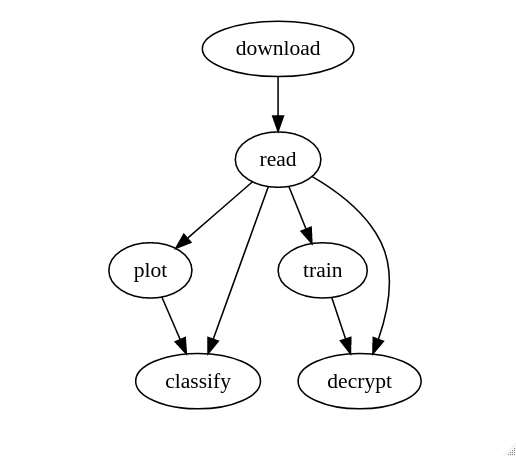
\includegraphics[width=0.6\linewidth]{imgs/fluxo} 

}

\caption{Fluxo de utilização do pacote `decryptr`.}\label{fig:fluxo}
\end{figure}

\subsection{Download}\label{download}

A função \texttt{download\_captcha()} tem cinco parâmetros:

\begin{itemize}
\tightlist
\item
  \texttt{url=} o link do CAPTCHA que queremos baixar.
\item
  \texttt{n=} a quantidade de CAPTCHAs a serem baixados.
\item
  \texttt{path=} a pasta que queremos salvar a imagem.
\item
  \texttt{secure=} se \texttt{TRUE}, fará o download com a opção
  \texttt{ssl\_verifypeer\ =\ FALSE}
  (\href{http://curso-r.com/blog/2017/03/31/2017-03-31-ssl/}{veja esse
  post})
\item
  \texttt{ext=} extensão do arquivo (\texttt{jpg}/\texttt{jpeg} ou
  \texttt{png}).
\end{itemize}

Para facilitar a utilização do \texttt{decryptr}, adicionamos algumas
atalhos do tipo \texttt{download\_captcha("nome")}, que já contêm os
padrões para download de alguns sites específicos:

\begin{itemize}
\tightlist
\item
  \texttt{download\_captcha("rfb")}:
  \href{http://www.receita.fazenda.gov.br/pessoajuridica/cnpj/cnpjreva/cnpjreva_solicitacao2.asp}{Consulta
  de CNPJ da Receita federal}.
\item
  \texttt{download\_captcha("saj")}:
  \href{https://esaj.tjsp.jus.br/cjsg/imagemCaptcha.do}{Sistema SAJ
  (vários Tribunais Estaduais)}.
\item
  \texttt{download\_captcha("tjmg")}:
  \href{http://www4.tjmg.jus.br/juridico/sf/captcha.svl}{Tribunal de
  Justiça de Minas Gerais}.
\item
  \texttt{download\_captcha("tjrj")}:
  \href{http://www4.tjrj.jus.br/consultaProcessoWebV2/captcha}{Tribunal
  de Justiça do Rio de Janeiro}.
\item
  \texttt{download\_captcha("tjrs")}:
  \href{http://www.tjrs.jus.br/site_php/consulta/human_check/humancheck_showcode.php}{Tribunal
  de Justiça do Rio Grande do Sul}.
\item
  \texttt{download\_captcha("trt")}:
  \href{https://pje.trt3.jus.br/consultaprocessual/seam/resource/captcha}{Tribunais
  Regionais do Trabalho}.
\end{itemize}

Exemplo:

\begin{Shaded}
\begin{Highlighting}[]
\KeywordTok{library}\NormalTok{(decryptr)}
\CommentTok{# salva arquivo em ./imgs/tjmg/captcha<id>.jpeg}
\NormalTok{arq <-}\StringTok{ }\KeywordTok{download_captcha}\NormalTok{(}\StringTok{"tjmg"}\NormalTok{, }\DataTypeTok{n =} \DecValTok{1}\NormalTok{, }\DataTypeTok{path =} \StringTok{'imgs/tjmg'}\NormalTok{) }
\end{Highlighting}
\end{Shaded}

\subsection{Visualização}\label{visualizacao}

Para plotar um CAPTCHA basta ler o arquivo com \texttt{read\_captcha()}
e depois usar a função \texttt{plot()}. Exemplo:

\begin{Shaded}
\begin{Highlighting}[]
\KeywordTok{library}\NormalTok{(decryptr)}
\StringTok{'imgs/tjmg/captcha2f6e4f7825d6.jpeg'} \OperatorTok\StringTok{ }
\StringTok{  }\KeywordTok{read_captcha}\NormalTok{() }\OperatorTok\StringTok{ }
\StringTok{  }\NormalTok{dplyr}\OperatorTok{::}\KeywordTok{first}\NormalTok{() }\OperatorTok\StringTok{ }
\StringTok{  }\KeywordTok{plot}\NormalTok{()}
\end{Highlighting}
\end{Shaded}

\begin{figure}
\centering
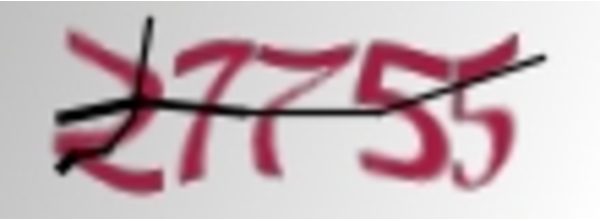
\includegraphics{jtrecenti_doctorate_captcha_files/figure-latex/unnamed-chunk-12-1.pdf}
\caption{\label{fig:unnamed-chunk-12}CAPTCHA do TJMG.}
\end{figure}

\subsection{Classificação}\label{classificacao}

A classificação manual de CAPTCHAs é importante para possibilitar o
treino de modelos preditivos. Para classificar um CAPTCHA você pode
utilizar a função \texttt{classify()}, assim:

\begin{Shaded}
\begin{Highlighting}[]
\StringTok{'imgs/tjmg/captcha2f6e4f7825d6.jpeg'} \OperatorTok\StringTok{ }
\StringTok{  }\KeywordTok{classify}\NormalTok{()}
\end{Highlighting}
\end{Shaded}

Essa função executa duas tarefas:

\begin{itemize}
\tightlist
\item
  Plota o CAPTCHA na tela.
\item
  Abre um console para o usuário digitar o valor do CAPTCHA manualmente.
\end{itemize}

Ao escrever o valor o CAPTCHA e pressionar
\texttt{\textless{}enter\textgreater{}}, a função \texttt{classify()}
adicionará a classificação no nome do arquivo da imagem. A função
\texttt{classify()} gera uma cópia para que seja impossível de perder a
imagem original.

Algumas opções do \texttt{classify()}:

\begin{itemize}
\tightlist
\item
  \texttt{answers=} adicionar uma resposta ao invés de esperar abrir o
  console. Essa opção é útil quando as classficações são feitas
  automaticamente (e.g., por um quebrador de CAPTCHAs que usa o áudio no
  lugar da imagem.)
\item
  \texttt{path=} colocar uma pasta para classificar os CAPTCHAs. Por
  padrão é a pasta onde os originais estão.
\end{itemize}

\subsection{Carregar modelo}\label{carregar-modelo}

A função \texttt{load\_model()} é responsável por carregar modelos pré
treinados

\begin{Shaded}
\begin{Highlighting}[]
\NormalTok{modelo <-}\StringTok{ }\NormalTok{decryptr}\OperatorTok{::}\KeywordTok{load_model}\NormalTok{(}\StringTok{"tjmg"}\NormalTok{)}
\NormalTok{modelo}\OperatorTok{$}\NormalTok{model}
\end{Highlighting}
\end{Shaded}

\subsection{Resolver captcha}\label{resolver-captcha}

A função \texttt{decrypt} resolve o CAPTCHA a partir de uma imagem e um
modelo.

\begin{Shaded}
\begin{Highlighting}[]
\KeywordTok{decrypt}\NormalTok{(}\StringTok{'imgs/tjmg/captcha2f6e4f7825d6.jpeg'}\NormalTok{, modelo)}
\CommentTok{#> "27755"}
\end{Highlighting}
\end{Shaded}

Também é possível chamar \texttt{decrypt} com o nome do modelo no lugar
do próprio modelo carregado.

\bibliography{bibliography/book.bib,bibliography/packages.bib}

\end{document}
